\documentclass{article}
\usepackage{graphicx} % Required for inserting images
\usepackage{float}
\usepackage[T1]{fontenc}
\usepackage{amsmath}
\usepackage[margin=1in]{geometry}
\usepackage{booktabs}
\usepackage{tabularx}
\usepackage[hidelinks]{hyperref}

\title{A learning-to-rank model that picks the put delta, or no trade, on the stress-sized put book}
\author{Experiment report \textperiodcentered{} L/S Gamma Desk, QUANTT}
\date{2026-11-05}

\begin{document}

\maketitle

\textbf{Question:} On the 35\% stress-sized \texttt{hedged} put book, does a LightGBM LambdaRank ranker built as in Wysocki (2026) give a higher Sharpe ratio than the fixed 25-delta put? The ranker is trained walk-forward from 2017 and each day picks the put delta (0.05-0.45) or no trade. The test is at 1x and 2x spreads, over the full window and in each half, within the stress budget and without a worse tail.

\textbf{Method:}

\begin{itemize}

\item \textbf{Pre-registered backtest:} the research switch was committed first (bbaa899), then the hypothesis card, config and script (7964782), before any run.

\item \textbf{Data:} R2 replay snapshots v1 (config\_hash b040760187f0), development window 2014-06-02 to 2024-12-31. The out-of-sample window (2025-01-01 to 2026-07-10) was not used.

\item \textbf{Book (every variant and the reference):} the \texttt{hedged} book of \texttt{2026-\allowbreak{}10-\allowbreak{}22-\allowbreak{}stress-\allowbreak{}sized-\allowbreak{}puts}.

\begin{itemize}

\item An always-on short put, with the signal ignored and the flat exit off.

\item Sized at entry so that a one-day 20\% SPY drop, with IV at max(60\%, the put's IV), costs at most 35\% of \$250k (\$87,500).

\item A 10-share daily hedge.

\item The 1x-credit stop, the 50\% profit-take, the 7-DTE time exit and the 1-day cool-off.

\end{itemize}

\item \textbf{New switch:} \texttt{[backtest] put\_\allowbreak{}picks} (default off) reads a file of daily picks. A pick sets that day's put delta target, and 0 means no entry; days without a pick use \texttt{put\_\allowbreak{}delta} (0.25).

\item \textbf{Labels:} for every development day and each of the 8 deltas (0.05, 0.10, 0.15, 0.20, 0.25, 0.30, 0.40, 0.45), an unregistered engine run opens that put at 10:15 and holds it under the book's rules until it first closes, at 1x spreads.

\begin{itemize}

\item The label is the paper's path score: net round-trip P\&L divided by the root sum of squared negative daily mark changes.

\item SKIP scores 0.

\item In total 20,376 labels on 2,547 days.

\end{itemize}

\item \textbf{Ranker:}

\begin{itemize}

\item LightGBM 4.7.0 \texttt{lambdarank}, gains [0, 1, 3, 7, 15], one query group per day.

\item A fixed list of 37 features: VIX family, realized vol, VRP, skew, term slope, days to FOMC and CPI, and each put's moneyness, IV, spread, size and Greeks per dollar of stress budget.

\item Fixed hyperparameters; early stopping on NDCG@1.

\end{itemize}

\item \textbf{Walk-forward:} retrained each year for test years 2017-2024. For year Y:

\begin{itemize}

\item the ranker fits on labels closed before Y \ensuremath{-} 9 months;

\item early stopping uses the next 3 months;

\item the confidence gate is calibrated on the last 6 months.

\end{itemize}

Each slice is purged so that no label overlaps the next.

\item \textbf{Gate:} the book abstains when the gap between the top two scores is below $\tau$. $\tau$ is chosen to maximise the Sortino ratio of the calibration slice's top-1 P\&L.

\item \textbf{Variants:}

\begin{itemize}

\item \texttt{ltr} (primary): the top pick, SKIP and the gate;

\item \texttt{ltr\_\allowbreak{}nogate}: the top pick with SKIP, no gate;

\item \texttt{ltr\_\allowbreak{}noskip}: the best-ranked put every day.

\end{itemize}

Before 2017 every variant trades the 25-delta put, so it matches the reference.

\item \textbf{Comparison:} the registered \texttt{2026-\allowbreak{}10-\allowbreak{}22-\allowbreak{}stress-\allowbreak{}sized-\allowbreak{}puts/\allowbreak{}hedged} runs (25-delta) at the same spread multiple, reused and not rerun.

\item \textbf{Runs and costs:}

\begin{itemize}

\item Every variant was run at 1x and 2x spreads, with picks trained on 1x labels.

\item Costs are \$0.65 per contract and \$0.005 per share, with a \$1 minimum per order.

\end{itemize}

\item \textbf{Timing:}

\begin{itemize}

\item Decisions, exits and hedges run at 10:15 ET.

\item Decisions read a 15-minute-old chain, and fills price on trades in the 15 minutes after.

\item Spot comes from put-call parity on the 30-minute snapshot grid (10:15-15:45).

\end{itemize}

\end{itemize}

This report was written by Claude at the PM's request.

\section{Result vs the pass bar}

Every check had to hold at 1x and 2x. P\&L is net of costs in USD for the whole sized book. Sharpe is annualised on \$250k. ES is the mean of the worst 5\% of daily P\&L.

\begin{center}\small
\begin{tabularx}{\linewidth}{>{\raggedright\arraybackslash}X l l l l l}
\toprule
\textbf{Check (\texttt{ltr} vs \texttt{hedged})} & \textbf{1x value} & \textbf{1x bar} & \textbf{2x value} & \textbf{2x bar} & \textbf{Result} \\
\midrule
Sharpe, full window & 0.84 & > 0.52 & 0.67 & > 0.43 & pass \\
Sharpe, 2014-06 to 2019-12 & 0.64 & > 0.84 & 0.43 & > 0.72 & \textbf{fail} \\
Sharpe, 2020-01 to 2024-12 & 1.09 & > 0.48 & 0.95 & > 0.38 & pass \\
Max drawdown \ensuremath{\leq} \$87,500 & \$14,810 & \ensuremath{\leq} \$87,500 & \$19,835 & \ensuremath{\leq} \$87,500 & pass \\
ES 5\% within 1.10x & \ensuremath{-}\$1,546 & \ensuremath{\geq} \ensuremath{-}\$3,317 & \ensuremath{-}\$1,566 & \ensuremath{\geq} \ensuremath{-}\$3,404 & pass \\
Event floor: round trips \ensuremath{\geq} 30 & 165 & \ensuremath{\geq} 30 &  &  & met \\
\bottomrule
\end{tabularx}
\end{center}

\textbf{Verdict: failed.}

\begin{itemize}

\item \texttt{ltr} has a higher full-window Sharpe, a far smaller drawdown and a milder tail, but its Sharpe is lower in 2014-2019 at both spreads.

\item It also makes less money: \$80k against \$121k at 1x, and \$64k against \$101k at 2x.

\item Most of its risk-adjusted gain comes from one decision: the gate abstained on every day from 19 February to 30 April 2020. The book was nearly flat through the COVID crash.

\end{itemize}

\subsection{Full-window numbers (not part of the bar)}

\texttt{ltr\_\allowbreak{}nogate} and \texttt{ltr\_\allowbreak{}noskip} are identical runs. The ranker put SKIP first on only 1 of 1,944 test days (28 July 2022), and the book was holding a put that day.

\begin{center}\small
\begin{tabularx}{\linewidth}{>{\raggedright\arraybackslash}X >{\raggedright\arraybackslash}X >{\raggedright\arraybackslash}X >{\raggedright\arraybackslash}X >{\raggedright\arraybackslash}X >{\raggedright\arraybackslash}X >{\raggedright\arraybackslash}X}
\toprule
\textbf{} & \textbf{hedged 1x} & \textbf{ltr 1x} & \textbf{ltr\_nogate 1x} & \textbf{hedged 2x} & \textbf{ltr 2x} & \textbf{ltr\_nogate 2x} \\
\midrule
Net P\&L & \$121,482 & \$80,124 & \$112,100 & \$101,172 & \$63,822 & \$105,115 \\
Sharpe & 0.52 & 0.84 & 0.55 & 0.43 & 0.67 & 0.51 \\
Max drawdown & \$70,362 & \$14,810 & \$52,803 & \$75,488 & \$19,835 & \$52,488 \\
ES 5\% (daily) & \ensuremath{-}\$3,016 & \ensuremath{-}\$1,546 & \ensuremath{-}\$2,523 & \ensuremath{-}\$3,094 & \ensuremath{-}\$1,566 & \ensuremath{-}\$2,554 \\
Round trips & 182 & 165 & 215 & 181 & 164 & 210 \\
Commissions (options /\allowbreak{} hedges) & \$5,955 /\allowbreak{} \$2,868 & \$5,392 /\allowbreak{} \$1,948 & \$7,205 /\allowbreak{} \$2,553 & \$5,918 /\allowbreak{} \$2,863 & \$5,392 /\allowbreak{} \$1,966 & \$7,047 /\allowbreak{} \$2,533 \\
\bottomrule
\end{tabularx}
\end{center}

\texttt{ltr\_\allowbreak{}nogate} (strike choice only) fails the same 2014-2019 check: Sharpe 0.53 against 0.84 at 1x, and 0.49 against 0.72 at 2x. Its full-window Sharpe is only slightly higher (0.55 against 0.52, and 0.51 against 0.43).

\section{Charts}

\begin{figure}[H]\centering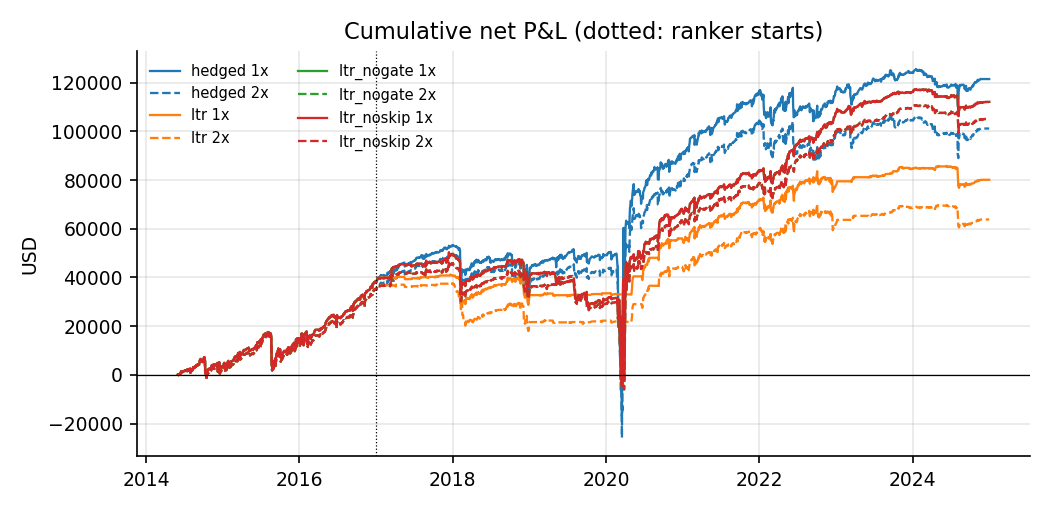
\includegraphics[width=0.92\linewidth]{figures/cum_pnl.png}\caption{Cumulative net P\&L, 1x solid and 2x dashed; ltr\_nogate is hidden under ltr\_noskip}\end{figure}

All books are identical through 2017-01-09 (\$39,304 at 1x; \$37,985 at the end of 2016). From 2017 to 2019 the ranker's books lose money while the reference gains. At 1x:

\begin{itemize}

\item \texttt{ltr} \ensuremath{-}\$4,481 and \texttt{ltr\_\allowbreak{}nogate} \ensuremath{-}\$7,239, against +\$11,147.

\end{itemize}

In 2020 the reference falls sharply and recovers. \texttt{ltr} barely moves, because it was out of the market. From 2021 the gaps are steady.

\begin{figure}[H]\centering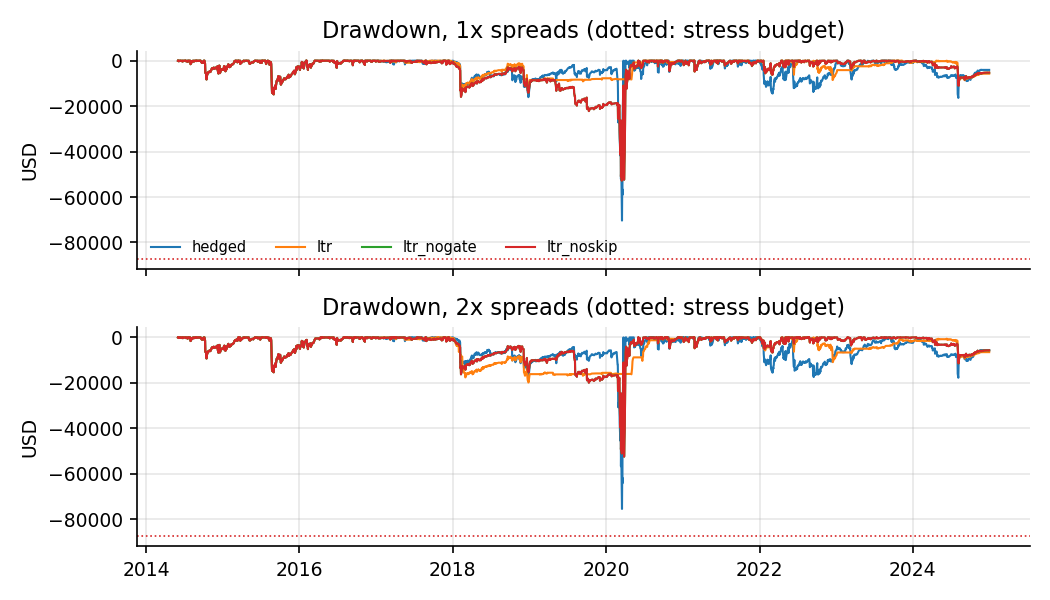
\includegraphics[width=0.92\linewidth]{figures/drawdown.png}\caption{Drawdown at 1x and 2x spreads (dotted: stress budget)}\end{figure}

The reference's largest drawdown runs from a January 2018 peak to the March 2020 trough (\$70.4k at 1x).

\texttt{ltr}'s worst drawdown at 1x is August 2015 (\$14.8k), before the ranker starts, so the reference has it too. At 2x it is \$19.8k, from December 2017 to December 2018.

\texttt{ltr\_\allowbreak{}nogate} still bottoms in March 2020. In 2020-2024 its worst drawdown is \$41.5k against the reference's \$67.6k, so lower deltas cut the crash loss by about 40\%. Avoiding the crash took the gate.

\begin{figure}[H]\centering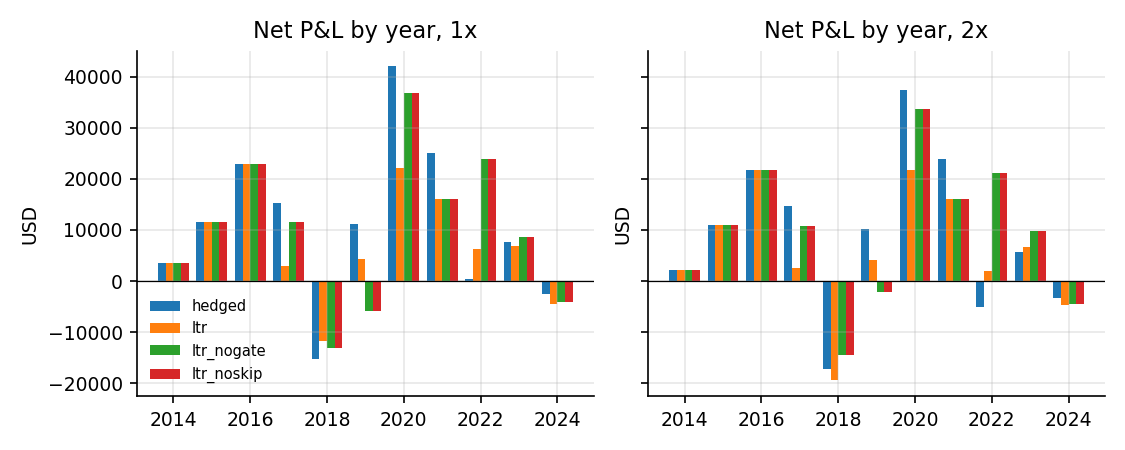
\includegraphics[width=0.92\linewidth]{figures/yearly.png}\caption{Net P\&L by year}\end{figure}

At 1x, \texttt{ltr} leads the reference only in 2018 (a smaller loss) and 2022, and trails in the other six test years; at 2x it leads in 2022 and 2023. \texttt{ltr\_\allowbreak{}nogate} leads only in 2018, 2022 and 2023.

The 2020 gap is the largest at 1x: \$22.1k (\texttt{ltr}) against \$42.0k.

\begin{figure}[H]\centering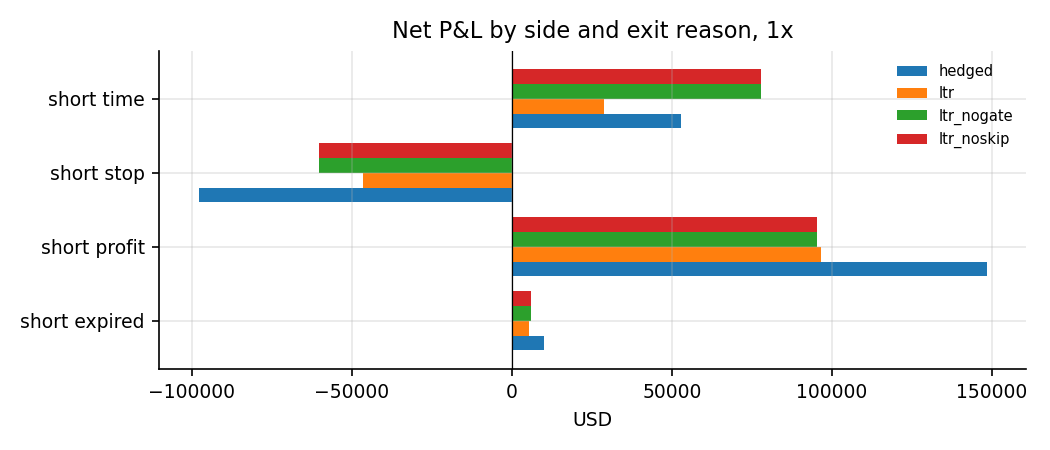
\includegraphics[width=0.92\linewidth]{figures/by_reason.png}\caption{Net P\&L by side and exit reason, 1x}\end{figure}

Lower-delta puts reach the 50\% profit-take more often and the 7-DTE time exit less often. From 2017, by book:

\begin{center}\small
\begin{tabularx}{\linewidth}{l l l l l >{\raggedright\arraybackslash}X}
\toprule
\textbf{Book} & \textbf{Round trips} & \textbf{Profit-takes} & \textbf{Time exits} & \textbf{Stops} & \textbf{Expired} \\
\midrule
\texttt{ltr} & 119 & 44 & 50 & 17 & 8 \\
\texttt{ltr\_\allowbreak{}nogate} & 169 & 52 & 89 & 22 & 6 \\
\texttt{hedged} & 136 & 13 & 115 & 7 & 1 \\
\bottomrule
\end{tabularx}
\end{center}

The reference's 8 stops cost \$97.9k over the whole window, \$57.7k of it in three stops in February-March 2020.

\begin{figure}[H]\centering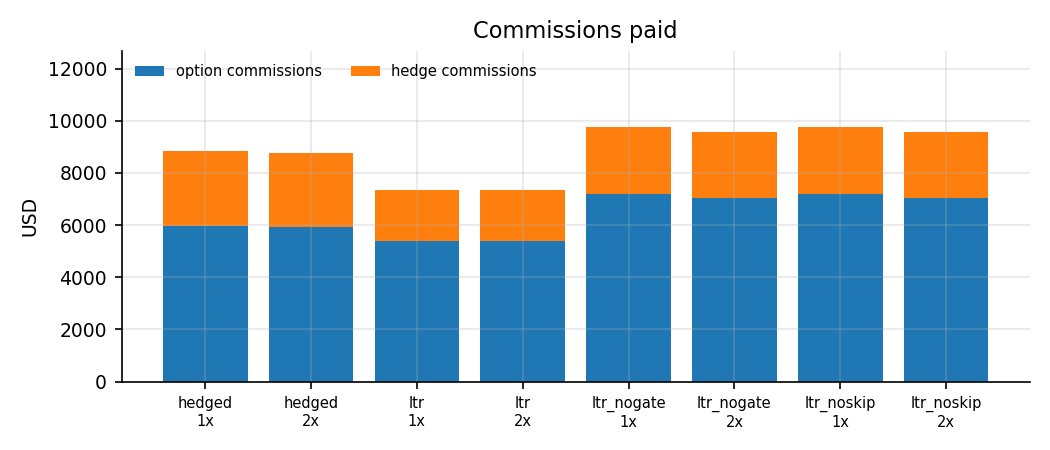
\includegraphics[width=0.92\linewidth]{figures/fees.png}\caption{Commissions paid}\end{figure}

Commissions are small in every book, between \$7.3k and \$9.8k over ten years. \texttt{ltr} pays the least because it trades less; \texttt{ltr\_\allowbreak{}nogate} pays the most because it has more, shorter round trips.

\begin{figure}[H]\centering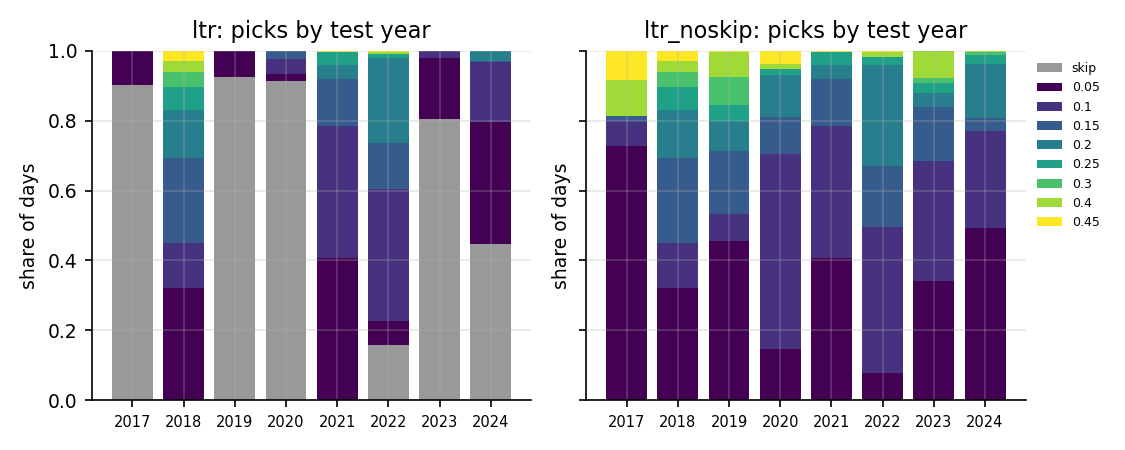
\includegraphics[width=0.92\linewidth]{figures/picks.png}\caption{Share of test days by pick, per test year: ltr (gate) and ltr\_noskip (best put)}\end{figure}

The ranker mostly picks far out-of-the-money puts: 5-delta on 37\% of test days and 10-delta on 28\%. 25-delta, the reference, gets 3\%.

The gate (grey) decides whole years:

\begin{center}\small
\begin{tabularx}{\linewidth}{l >{\raggedright\arraybackslash}X}
\toprule
\textbf{Test year} & \textbf{Days \texttt{ltr} would trade} \\
\midrule
2017 & 10\% \\
2018 & 100\% \\
2019 & 7\% \\
2020 & 9\% \\
2021 & 100\% \\
2022 & 84\% \\
2023 & 20\% \\
2024 & 55\% \\
\bottomrule
\end{tabularx}
\end{center}

\begin{figure}[H]\centering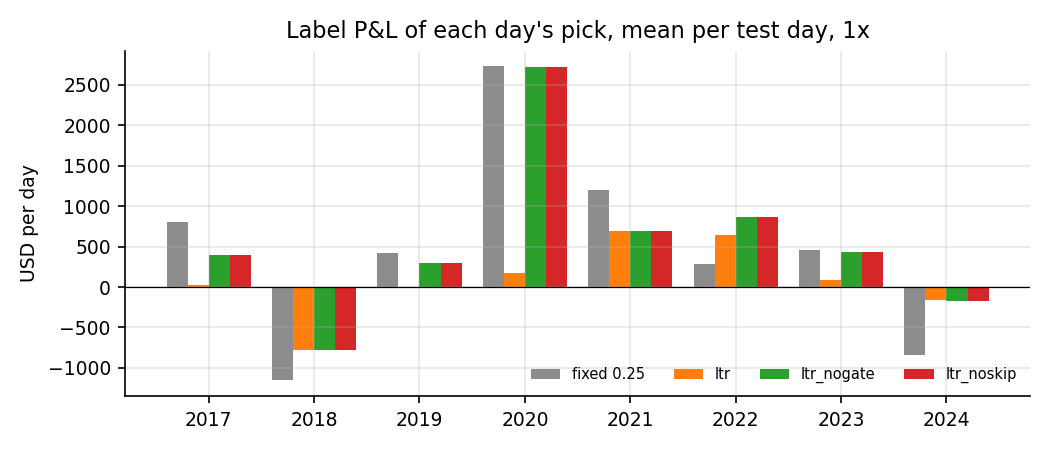
\includegraphics[width=0.92\linewidth]{figures/ranking.png}\caption{Mean label P\&L per test day of each variant's pick, against always picking the 25-delta put, 1x}\end{figure}

This chart scores the picks at the label level: every test day's pick, not just the days the book was flat.

\begin{itemize}

\item The best-put picks average \$557 a day against \$490 for the 25-delta put.

\item On the 1,915 days where both have a label, the edge is \$69 a day, but it isn't reliable: t = 0.57 on monthly means, and only 41\% of 95 months are positive.

\end{itemize}

\begin{figure}[H]\centering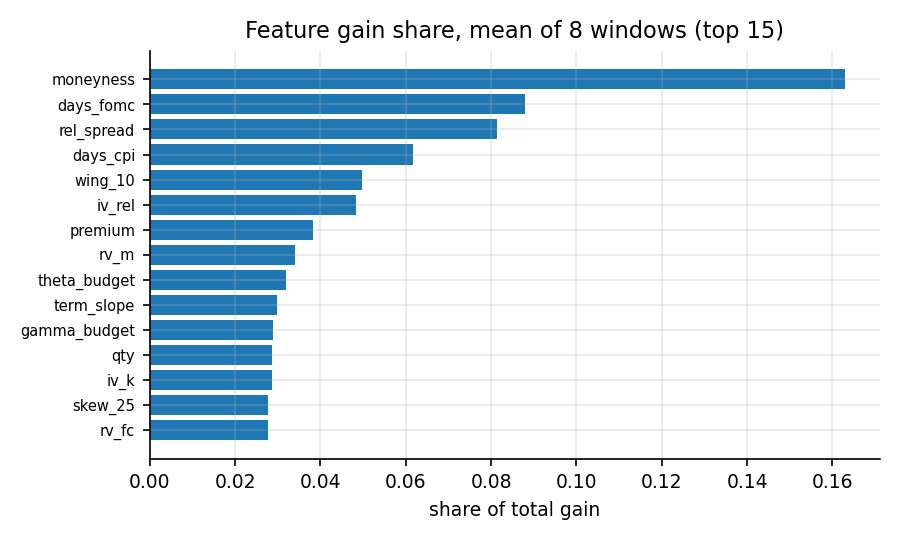
\includegraphics[width=0.92\linewidth]{figures/importance.png}\caption{Feature gain share, mean of the 8 windows (top 15)}\end{figure}

Features of the put itself carry half the gain (50\%), led by moneyness (16\%) and relative spread (8\%). Days to FOMC and CPI carry 15\% together. VRP carries 1.3\%.

\section{Analysis}

\subsection{The gate, not the ranking, drives the result}

\begin{itemize}

\item The ranker put SKIP first on only 1 test day, so \texttt{ltr} skipped only through the gate: 603 entry days.

\item $\tau$ was set by each window's calibration half-year, and the trade rate swung from 7\% to 100\% between adjacent years. The book was in the market:

\begin{itemize}

\item 35-38\% of days in 2017, 2019 and 2020;

\item 97-99\% in 2018, 2021 and 2022.

\end{itemize}

\item 2020's $\tau$ came from the second half of 2019 (it traded 11.5\% of those days). It abstained on all 49 days from 19 February to 30 April 2020. The book was in the market on 6\% of those days and lost \$151, against +\$21.7k for the reference, whose \$70.4k maximum drawdown bottomed in that window (\$66.8k peak to trough inside it).

\item Outside that window, the full-window Sharpe ratios are close: 0.85 for \texttt{ltr} against 0.81 for \texttt{hedged} at 1x, and 0.68 against 0.66 at 2x.

\item The gate's 2020 trading days were 21 of 244, none of them in the crash window. That is suggestive, but trading days cluster, so the evidence is weak. The gate was not crash-aware by design: it was simply selective all year.

\end{itemize}

\subsection{Where the book traded, the strike choice did not beat 25-delta}

\begin{itemize}

\item In 2017-2019 the ranker's books lost money (\ensuremath{-}\$4.5k for \texttt{ltr}, \ensuremath{-}\$7.2k for \texttt{ltr\_\allowbreak{}nogate} at 1x) while the reference made \$11.1k.

\item In the walk-forward test years, the ranker does better than chance on its own target: its pick was the day's best put 25\% of the time, against 12.5\% by chance and 6\% for the 25-delta. Its mean grade was 1.88 against 1.81 for the 25-delta.

\item The label score rewards smooth paths, though, and 5-delta puts have them (40\% reach the profit-take) while earning the least: \$35 per label on average against \$607 for 25-delta.

\item So the ranker's taste for 5- and 10-delta puts gives quick small wins, not more P\&L. From 2017, \texttt{ltr}'s 57 entries at 5-delta made \$4.4k in total, against \$33.9k from its 13 entries at 15-delta.

\end{itemize}

\subsection{The sample is thin, and the boosting is shallow}

\begin{itemize}

\item Early stopping on about 42 days of NDCG@1 kept every model small: 3 to 45 boosting rounds.

\item Consecutive days' labels share most of their path, so the 2,547 labelled days hold far fewer independent outcomes. The book itself makes only 119-169 entries from 2017.

\item A few large outcomes per year decide the comparison, as August 2015 did for the 20-delta card.

\end{itemize}

\subsection{Mechanical effects}

\begin{itemize}

\item Far out-of-the-money puts often have no fill price near expiry, so the close fails and the put is held to settlement. There were 52 failed close attempts on 10 \texttt{ltr} puts (9 of which expired), 36 on 8 \texttt{ltr\_\allowbreak{}nogate} puts (7 expired), and 9 on 2 reference puts (both expired).

\item That favours low deltas in calm markets: the credit is kept. It would hurt in a crash, because a stop also needs a fill.

\end{itemize}

\section{Verdict}

\textbf{Failed} per the pre-registered bar: Sharpe is lower in 2014-2019 at 1x and 2x.

The higher full-window Sharpe and the small drawdown come mostly from a gate that happened to sit out the 2020 crash, at the cost of a third less P\&L. The ranker's strike choice alone (\texttt{ltr\_\allowbreak{}nogate}) is close to the fixed 25-delta book and fails the same check.

Next step: archive this card, and don't run the out-of-sample test.

A follow-up would need its own card. Two options:

\begin{itemize}

\item a P\&L-based label instead of the path score;

\item a gate tested on its own as a crash filter, e.g. how often a fixed-$\tau$ gate would have been flat in other selloffs (August 2015, February 2018, Q4 2018). That needs a design that does not peek at 2020.

\end{itemize}

\section{Caveats}

\begin{itemize}

\item \textbf{In-sample:} the book was chosen after its 2014-2024 results, and the desk had seen results by delta (15, 20, 25, 35, ATM) before this card. The walk-forward keeps each year's picks out of its own training, but not the design.

\item \textbf{One episode:} most of the Sharpe and drawdown gap is the 2020 crash window (49 days).

\item \textbf{Departures from the paper:}

\begin{itemize}

\item 30-DTE SPY puts held to the book's exits, not 0DTE SPXW held to settlement;

\item daily bars and net P\&L in the label;

\item fixed hyperparameters, with no Optuna search;

\item a fixed feature list, with no S1-S5 selection;

\item no put-call ratios;

\item stress-budget sizing.

\end{itemize}

\item \textbf{Fills:} low-delta puts often lack fill prices near expiry, so they are held to settlement (see Analysis).

\item \textbf{Spread model:} fitted on about two weeks of calm 2026 live quotes; fills of up to 81 contracts in the ranker books (100 in the reference) use the one-contract model. The 2x run is the stress test.

\item \textbf{Data gaps:} about 3.3\% of scheduled times are skipped (no snapshot), as in every run.

\end{itemize}

\section{Trials}

6 trials for this experiment (3 variants \ensuremath{\times} 1x and 2x, one run of \texttt{experiment.\allowbreak{}py}), all tagged with the pre-registration commit 7964782. The \texttt{hedged} reference and the baseline were reused, not rerun; the registry now has 140 rows and none out of sample.

The run was started three times; only the third registered trials:

\begin{itemize}

\item \textbf{First attempt:} stopped while building labels, because another process switched the shared working tree to \texttt{main}, which removed this card's config.

\item \textbf{Second attempt:} stopped by Claude while building labels, because 12 worker processes each started a 14-thread pool, which oversubscribed the machine.

\item \textbf{Third attempt:} ran from a separate checkout of the branch with one thread per worker (an environment setting; the code did not change). It registered the 6 trials, then crashed in one chart (a duplicate index in the picks chart). That chart was fixed in \texttt{experiment.\allowbreak{}py} and the report rebuilt from the saved runs in report-only mode, which adds no trials.

\end{itemize}

Neither of the first two attempts produced labels or registered trials. The pass bar was not changed.

\end{document}
